\chapter{Fundamentals}
\label{ch:fundamentals}

This chapter introduces the ideas and methods the rest of the thesis builds on. It is written for a reader with a computer-science background who has not worked in music information retrieval (MIR) or machine learning before. Sections~\ref{sec:fund_emotion_def} to \ref{sec:fund_motivation_theory} cover the topic itself. They explain what ``emotion'' means when a machine has to predict it, how emotion in music is modelled, and why emotion should tell us anything about film genre. Sections~\ref{sec:fund_audio} to \ref{sec:fund_evaluation} cover the tools. They show how audio is turned into numbers a model can use, which learning methods are used and why, and how the results are measured so that later comparisons are fair.

\section{Defining ``Emotion'' in a Machine Learning Context}
\label{sec:fund_emotion_def}

In this thesis, ``emotion'' does not mean a state inside the trained model, and the system does not ``feel'' anything. In the music emotion recognition (MER) literature, ``music emotion'' is short for \emph{emotion perceived in music} \citep{yang2012machine}. It is a listener's judgement of what a piece of music expresses, not what the listener feels while hearing it.

\citet{gabrielsson2002emotion} was the first to set out this distinction carefully. \emph{Perceived} emotion is what the music is judged to express. \emph{Induced} or \emph{felt} emotion is what the listener experiences. The two are related, but studies show they can come apart. The dataset used in this thesis \citep{eerola2011comparison} measures only perceived emotion. Listeners rated what each film-music clip expressed, not how it made them feel.

This matters for how the system should be understood. The model does not learn an emotional state. It learns to map acoustic features onto a number, and that number is itself an average of human judgements. ``Emotion'' here is therefore a measured label: the mean of several listeners' ratings on a fixed scale. The models of Chapter~\ref{ch:methods} are trained to reproduce this human target. Nothing in them is an emotional process of its own.

In practice, each clip in the dataset has eight numbers between 1 and 9. Three are continuous scales: \emph{valence} (unpleasant to pleasant), \emph{energy arousal} (calm to energetic) and \emph{tension arousal} (relaxed to tense). The other five say how strongly a named emotion is present: \emph{anger}, \emph{fear}, \emph{happiness}, \emph{sadness} and \emph{tenderness}. A clip from a horror score might, for example, be rated 2.1 for valence, 7.8 for tension and 7.5 for fear, and close to 1 for happiness and tenderness. These eight numbers are what this thesis means by ``emotion''. The next section discusses the two frameworks they come from.

\section{Dimensional versus Categorical Emotion Models}
\label{sec:fund_models}

Research on emotion in music mostly uses one of two frameworks: the \emph{dimensional} model and the \emph{categorical} (or discrete) model.

\subsection{The Dimensional Model}

The dimensional model places an emotion at a point in a continuous space. Usually the space has two axes: \emph{valence}, how positive or negative an emotion is, and \emph{arousal}, how activated or calm it feels. The best-known version is the circumplex model of affect by \citet{russell1980circumplex}. Here ``happy'' is not a category of its own but the part of the space with high valence and fairly high arousal. ``Sad'' is low on both, and ``angry'' is low valence with high arousal. Much MER research has used this two-dimensional framework (surveyed in \citealp{kim2010music} and \citealp{kang2025there}). One reason is that it is comparatively easy to annotate and to model as a continuous regression target. Figure~\ref{fig:circumplex} sketches the space, with the five discrete emotions rated in the dataset used here.

\begin{figure}[t]
  \centering
  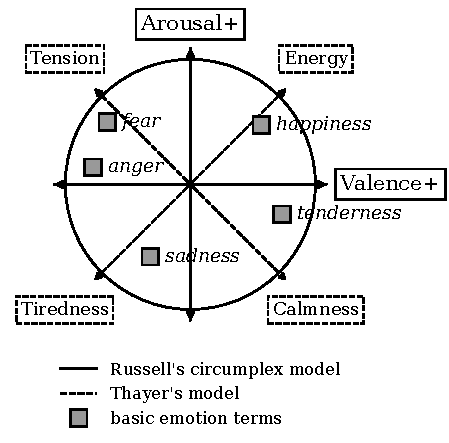
\includegraphics[width=0.62\textwidth]{figures/circumplex.pdf}
  \caption{The emotion space, adapted from Figure~1 of \citet{eerola2011comparison}.}
  \label{fig:circumplex}
\end{figure}

In Figure~\ref{fig:circumplex}, the solid axes are valence and arousal, as in the circumplex of \citet{russell1980circumplex}. The dashed diagonals are the two kinds of arousal that \citet{eerola2011comparison} rate separately: energy, from tiredness to energy, and tension, from calmness to tension. The original credits this pair of axes to the model of activation of \citet{thayer1989biopsychology}, as the key below the circle shows. Together with valence, they are the three dimensional scales used in this thesis. The grey squares mark the five discrete emotions of the dataset. The original drawing also shows surprise and disgust, which the dataset does not rate. It has no square for happiness, which is added here in the pleasant, energetic quadrant. The drawing shows the three dimensions at right angles, but the original notes that real ratings need not look like this. In the dataset used here, energy and tension correlate at $r=0.58$, and valence and tension at $r=-0.91$ (Appendix~\ref{sec:app_ratings}). Anger and fear share the unpleasant, high-arousal quadrant, so valence and arousal alone put them close together.

\subsection{The Categorical Model}

The categorical model describes emotion with a small set of labels instead, such as anger, fear, happiness, sadness and tenderness. Its advantage is that these labels match the words people use for emotions every day. Its difficulty is deciding how many categories are needed, and which ones, to describe emotion in music well.

\subsection{How the Two Models Relate}
\label{subsec:fund_why_not_va}

Two findings bear on how the two frameworks relate to each other.

\paragraph{Energetic and tense arousal are empirically distinct dimensions.} \citet{schimmack2002experiencing} tested whether energetic and tense arousal can be reduced to valence plus a single arousal factor. Once the variance shared with valence was removed, the remaining correlation between the two was not significantly different from zero. They are two separate dimensions, not one. This is the psychological basis for the three-dimensional model of \citet{eerola2011comparison} (valence, energy arousal, tension arousal).

\paragraph{Hybrid theoretical models support combining both frameworks.} \citet{eerola2011comparison} themselves report that, for averaged listener ratings, their three-dimensional model can be reduced linearly to two dimensions without a significant loss of fit. They also find that the five discrete emotions match regions of this two-dimensional space closely. For a model that predicts from such ratings, the two frameworks therefore carry largely the same information. They differ in what they let a person read off the model. This fits hybrid accounts of emotion (discussed in \citealp{eerola2011comparison}). In these accounts, core affect is dimensional, while putting a name to an emotional episode draws on further categorical or appraisal information that the dimensional space does not hold.

\section{Theoretical Motivation: Why Should Emotion Predict Genre?}
\label{sec:fund_motivation_theory}

The starting observation of this thesis is that soundtracks of different genres tend to sound emotionally different. This is more than a statistical regularity in the data. It reflects a known, deliberate practice in film scoring.

\citet{gorbman1987unheard} argues that film music works through an established system of musical codes. Minor keys and dissonant harmonies have come to signal threat or suspense. Other choices of harmony and instruments are linked to romance, comedy or heroism. Composers use these codes deliberately, to steer what the audience expects in line with the film's genre.

\citet{juslin2013everyday} places this within a broader account of how music conveys and arouses emotion. In his account, mechanisms such as learned association let music call up emotional meanings that a culture has settled on. In film scoring these meanings are often bound to genre conventions. Driving, dissonant and tense cues, for example, are conventional in horror and action scores.

This motivates the method. The related work in Chapter~\ref{ch:relatedwork} treats the link between audio and genre as a purely statistical pattern-recognition problem. It predicts genre straight from audio features and does not ask why audio should predict genre at all. I instead treat emotion as a possible reason for that link. Film composers put emotional signals that suit the genre into the score, and a model may be able to recover and use them. From this perspective, emotion is more than a convenient intermediate step for better predictions. It is a hypothesis about how a film's soundtrack comes to signal its genre.

\section{From Audio to Numbers: Representations}
\label{sec:fund_audio}

A learning algorithm cannot operate on an audio file directly. A ten-second clip at 16\,kHz is a sequence of 160{,}000 sample values, and two clips that sound alike can differ in every one of them. Any audio system therefore first turns the signal into a fixed-length vector of numbers, so that clips that sound alike lie close together. Such a vector is called a \emph{representation}, or in this thesis an \emph{embedding}. All later steps operate on these vectors, so the representation limits what any later model can learn.

\subsection{The Spectrogram}

Almost every audio representation starts from the \emph{spectrogram}. The signal is cut into short overlapping windows (typically 10--25\,ms). For each window, a Fourier transform measures how much energy lies at each frequency. Stacking the windows gives a two-dimensional image, with time on one axis and frequency on the other. Two refinements are standard. The frequency axis is mapped onto the \emph{mel} scale, which spaces frequencies the way human hearing does: finer at low pitches, coarser at high ones. The energies are also put on a logarithmic scale, because perceived loudness grows roughly logarithmically with energy. The result, the \emph{log-mel spectrogram}, is the input to four of the five learned models used here. It drops phase and fine timing below the window length. In this way it keeps roughly the information that the ear keeps, which is one reason for its wide use. Figure~\ref{fig:spectrogram} shows both forms for one clip of the dataset used here.

\begin{figure}[!htb]
  \centering
  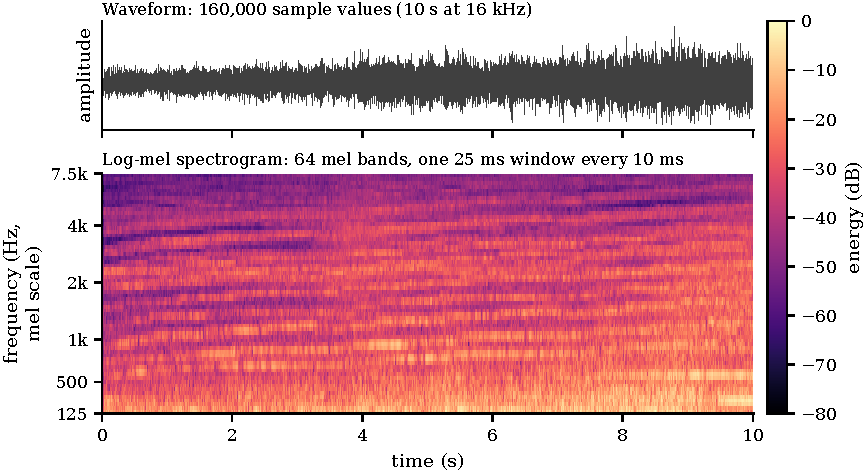
\includegraphics[width=\textwidth]{figures/spectrogram.pdf}
  \caption{Waveform and log-mel spectrogram of a film-music clip.}
  \label{fig:spectrogram}
\end{figure}

The clip in Figure~\ref{fig:spectrogram} comes from the score of the Horror film \emph{Hellraiser}, and its listeners rated it among the most fearful of the Horror clips. The waveform at the top holds 160{,}000 values. The spectrogram below it holds one value per mel band and 10\,ms step, with brighter colours for more energy. Its settings are those of the VGGish front end: 64 mel bands between 125\,Hz and 7.5\,kHz, and windows of 25\,ms.

\subsection{Hand-crafted Features}

The classical approach in MIR summarises the spectrogram with descriptors designed by hand. The spectrogram here is computed by a short-time Fourier transform (STFT). Typical descriptors are mel-frequency cepstral coefficients (MFCCs, a compact description of timbre), the spectral centroid (the ``centre of mass'' of the spectrum, which goes with brightness), the zero-crossing rate, chroma (how the energy spreads over the twelve pitch classes) and tempo. Each is computed per window and then summarised over time by its mean and standard deviation. Their strength is that they are transparent: each number has a known meaning. Their weakness is that they capture only the properties their designers chose to measure.

\subsection{Learned Embeddings from Pretrained Networks}

The alternative is to let a neural network learn the representation. The network is first trained for some task on a very large labelled audio dataset. A network is a stack of layers, and the output of each layer is called a \emph{hidden state}. After training, the hidden state of one inner layer serves as a general description of any new audio, whether or not it looks like the training data. This is called \emph{transfer learning}. The network is not retrained for the new task, and this output vector is the embedding. A network trained on millions of sounds tends to encode properties such as instrumentation, texture and dynamics in its inner layers. These carry over well to tasks it was never trained for \citep{choi2017transfer}. The output is averaged over time (\emph{mean-pooled}) to get one vector per clip.

I use five such networks:

\begin{itemize}
  \item \textbf{VGGish} \citep{hershey2017cnn} runs a convolutional network, of the kind first built for images, over log-mel patches. It was trained on a large collection of YouTube videos (an early version of the YouTube-8M dataset) and is distributed with the AudioSet release. It gives 128 numbers per clip.
  \item \textbf{AST} \citep{gong2021ast}, the Audio Spectrogram Transformer, treats the spectrogram as an image cut into patches. It then applies a Transformer, the attention-based architecture behind modern language models, across these patches. It was trained on AudioSet, two million YouTube clips labelled with 527 sound categories, music among them. It gives 768 numbers per clip. The recent survey by \citet{kang2025there} counts it among the large pretrained audio encoders that may make up for how small emotion-annotated datasets are.
  \item \textbf{CLAP} (Contrastive Language--Audio Pretraining) \citep{wu2023clap} is trained to match audio with text descriptions. Its embedding space is therefore organised by what a sound would be called. It gives 512 numbers per clip.
  \item \textbf{MusiCNN} \citep{pons2019musicnn} is the only one trained on music alone. It learned to predict descriptive tags for songs in the Million Song Dataset (MSD) and gives 200 numbers per clip. Several of its tags are mood words.
  \item \textbf{wav2vec 2.0} \citep{baevski2020wav2vec} does not start from a spectrogram. It applies convolutions straight to the raw samples, with no Fourier transform, and was trained on speech. It gives 768 numbers per clip.
\end{itemize}

The single dimensions of these embeddings have no fixed meaning. Dimension 87 of a VGGish vector encodes some property of the audio. Nothing guarantees, however, that it encodes the same property in another dataset, and a person cannot interpret it. The eight emotion ratings are different, because each one means the same everywhere. This is why the emotion representation is worth studying for more than its accuracy.

\section{Machine Learning Background}
\label{sec:fund_ml}

\subsection{Supervised Learning, Regression and Classification}

All models in this thesis are \emph{supervised}. They are shown inputs together with the correct outputs and adjust their internal parameters until they can reproduce the outputs from the inputs. The hope is that a model that does this well on the examples it has seen will also do well on new ones, that is, that it \emph{generalises}. Whether it does is what the evaluation has to test, and the whole evaluation procedure of Section~\ref{sec:fund_evaluation} exists to measure it.

Two kinds of task appear in this thesis. When the output is a number on a continuous scale, such as an emotion rating between 1 and 9, the task is \emph{regression}. When the output is a category, for instance whether a clip comes from an Action film, the task is \emph{classification}. The pipeline uses one of each, one after the other. A regressor maps the audio to the eight emotion values, and a classifier maps these values to genre.

\subsection{Multi-label Classification}

A film can belong to several genres. \emph{Gladiator}, for example, is Action, Adventure and Drama at once. Genre prediction is therefore \emph{multi-label}: the target is not a single class but a binary vector with one entry per genre, and several entries can be 1. It is handled with \emph{binary relevance}, the simplest principled approach. One independent binary classifier is trained per genre, and their outputs are combined into one label vector.

\subsection{The Two Models Used}

\paragraph{Logistic regression} is the genre classifier. For each genre it learns one weight per input feature. The logistic function maps the weighted sum of the features to a probability, and the clip is assigned the genre if this probability exceeds one half. It is linear and fast. Above all, it is interpretable: the weight on ``fear'' in the Horror classifier can be looked up and reported. With eleven emotion features it has eleven weights per genre. With a 768-dimensional embedding it has 768.

The number of weights matters because of \emph{overfitting}. With 768 adjustable weights and only about 330 clips, four fifths of which are in each training fold, a model can fit the training data almost perfectly. It does so by fitting chance correlations that do not recur in new data. The model then memorises the training data instead of learning a general relation. The usual remedy is \emph{regularisation}. A penalty on large weights is added to what the model minimises, which favours simpler solutions. One hyperparameter sets its strength, called $C$ in the implementation used. A small $C$ means strong regularisation.

\paragraph{Random forest} is the emotion regressor. It grows several hundred decision trees, each on a random part of the training data and features, and averages their predictions. Each tree splits the input space by tests such as ``is feature 41 greater than 0.3?'', so a forest can model relations that are not linear. Unlike a linear regressor, a forest also needs no regularisation strength to be tuned.

\paragraph{Two alternatives for the emotion regressor} are compared in Chapter~\ref{ch:evaluation}. \emph{Ridge regression} is ordinary linear regression with the same kind of penalty on large weights as above, so it predicts each rating as a weighted sum of the features. \emph{Support vector regression} (SVR) works differently. It ignores errors smaller than a set margin and only penalises larger ones, which keeps it robust to small noise in the ratings. With a \emph{radial basis function} (RBF) kernel, it predicts a rating from how similar a new clip is to selected training clips, where similarity falls off with the distance between their embeddings. Like the random forest, it can therefore model relations that are not linear.

\subsection{The Emotion Bottleneck}
\label{subsec:fund_bottleneck}

The central idea of the thesis can now be stated. The \emph{direct} approach feeds the audio embedding (128 to 768 numbers) straight into the genre classifier. The \emph{two-stage} approach first predicts the eight emotions from the embedding. Only these eight numbers, plus three simple combinations of them, reach the classifier. Everything the classifier learns about the audio has to pass through eight emotion values. In machine learning, such a deliberately narrow channel is called a \emph{bottleneck}.

A bottleneck discards information, so it can only help if the information it retains is more useful than the information it discards. I hypothesise that this bottleneck retains the information relevant to genre and discards the rest. I further hypothesise that it does so in a way a generic compression cannot, because its eight dimensions are quantities people can understand, and they mean the same in any dataset. A generic compression, such as principal component analysis (PCA), keeps the directions of largest variance in the data, whatever they mean. Comparing the bottleneck with such a compression of the same size separates the effect of its meaning from the effect of its size (Section~\ref{sec:methods_baselines}).

\section{Measuring Model Performance}
\label{sec:fund_evaluation}

\subsection{Cross-validation, and Why It Must Be Grouped by Film}

A model's performance on its own training data says little about how it generalises. The standard remedy is \emph{cross-validation}. The data are split into $k$ parts of about equal size, called \emph{folds}. In each \emph{round}, the model is trained on $k-1$ folds and scored on the one left out, and this is repeated until every fold has been the test set once. The average test score estimates how the model will do on new data.

On this dataset a naive split is invalid, and the resulting error can be measured. The 346 clips come from only 42 films. Clips from the same film share instruments and recording quality, and by definition also their genre label. If one clip from \emph{Gladiator} is in the training set and another in the test set, the model can score well on the test clip by recognising \emph{Gladiator} rather than Action. I therefore group every split \emph{by film}: all clips of a film stay on the same side. Figure~\ref{fig:grouped_cv} illustrates this for five folds, and Section~\ref{sec:evaluation_protocol} reports how large the effect of grouping is on the data used here.

\begin{figure}[!htb]
  \centering
  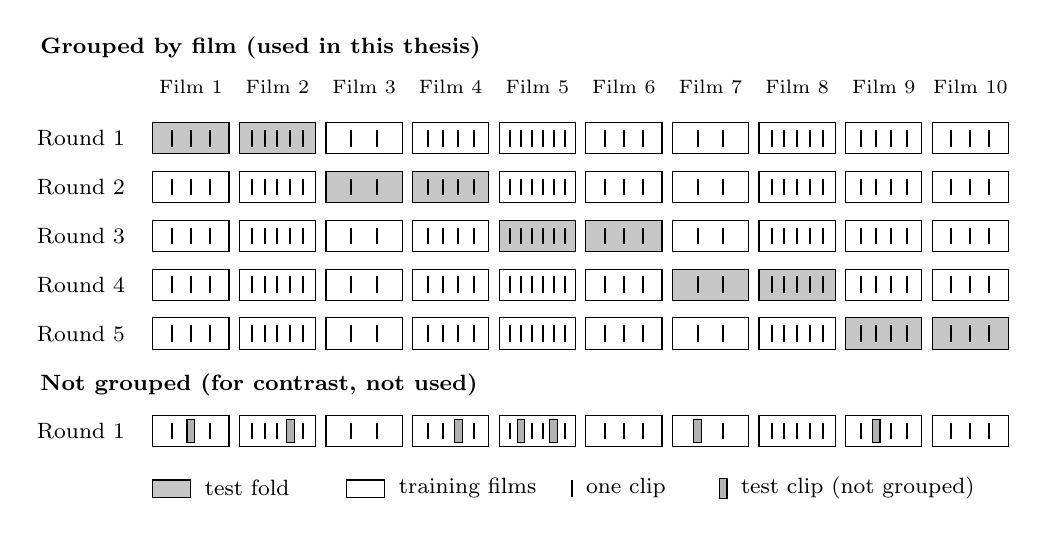
\begin{tikzpicture}[x=1.1cm, y=0.62cm, font=\footnotesize]
    % grouped by film: five rounds, one fold of two films is tested in each
    \node[anchor=west, font=\footnotesize\bfseries] at (-1.35,0.85) {Grouped by film (used in this thesis)};
    \foreach \film in {1,...,10} {\node at (\film-0.5,0.05) {\scriptsize Film \film};}
    \foreach \row in {1,...,5} {
      \node[anchor=east] at (-0.15,-\row) {Round \row};
      \foreach \pos/\nclips in {0/3,1/5,2/2,3/4,4/6,5/3,6/2,7/5,8/4,9/3} {
        \pgfmathtruncatemacro{\fold}{int(\pos/2)+1}
        \ifnum\fold=\row
          \draw[fill=gray!45] (\pos+0.06,-\row-0.32) rectangle (\pos+0.94,-\row+0.32);
        \else
          \draw (\pos+0.06,-\row-0.32) rectangle (\pos+0.94,-\row+0.32);
        \fi
        \foreach \clip in {1,...,\nclips} {
          \pgfmathsetmacro{\xx}{\pos+0.06+0.88*\clip/(\nclips+1)}
          \draw[line width=0.7pt] (\xx,-\row-0.17) -- (\xx,-\row+0.17);
        }
      }
    }
    % contrast: clips assigned to folds one by one, so test clips sit inside training films
    \node[anchor=west, font=\footnotesize\bfseries] at (-1.35,-6.05) {Not grouped (for contrast, not used)};
    \node[anchor=east] at (-0.15,-7) {Round 1};
    \foreach \pos/\nclips in {0/3,1/5,2/2,3/4,4/6,5/3,6/2,7/5,8/4,9/3} {
      \draw (\pos+0.06,-7.32) rectangle (\pos+0.94,-6.68);
      \foreach \clip in {1,...,\nclips} {
        \pgfmathsetmacro{\xx}{\pos+0.06+0.88*\clip/(\nclips+1)}
        \draw[line width=0.7pt] (\xx,-7.17) -- (\xx,-6.83);
      }
    }
    \foreach \pos/\nclips/\clip in {0/3/2,1/5/4,3/4/3,4/6/2,4/6/5,6/2/1,8/4/2} {
      \pgfmathsetmacro{\xx}{\pos+0.06+0.88*\clip/(\nclips+1)}
      \draw[fill=gray!60, draw=black, line width=0.4pt] (\xx-0.045,-7.24) rectangle (\xx+0.045,-6.76);
    }
    % key
    \draw[fill=gray!45] (0.06,-8.35) rectangle (0.5,-8.0);
    \node[anchor=west] at (0.55,-8.17) {test fold};
    \draw (2.3,-8.35) rectangle (2.74,-8.0);
    \node[anchor=west] at (2.79,-8.17) {training films};
    \draw[line width=0.7pt] (4.9,-8.35) -- (4.9,-8.0);
    \node[anchor=west] at (4.95,-8.17) {one clip};
    \draw[fill=gray!60, draw=black, line width=0.4pt] (6.6,-8.38) rectangle (6.69,-7.97);
    \node[anchor=west] at (6.74,-8.17) {test clip (not grouped)};
  \end{tikzpicture}
  \caption{Five-fold cross-validation grouped by film.}
  \label{fig:grouped_cv}
\end{figure}

In Figure~\ref{fig:grouped_cv}, ten films are divided into five folds of two films each. Each mark inside a film stands for one of its clips, and the films differ in their number of clips, as they do in the real data. Each of the upper rows is one round: one fold, shown in grey, is the test data, and the other four folds are the training data. Over the five rounds every film is tested exactly once. A film is never divided, so no clip of a test film is seen in training. The bottom row shows, for contrast, a split that is not grouped and is not used here. There the clips are assigned to folds one by one, so the test clips, shown as grey bars, come from films whose other clips are in training.

Two refinements are common. The assignment of items to folds can be reshuffled and the cross-validation repeated, which gives more test scores and a more stable estimate. Hyperparameters, such as the regularisation strength $C$, can be chosen by a second, \emph{inner} cross-validation inside each training fold, so that the test fold never affects the choice. This is called \emph{nested} cross-validation.

\subsection{Metrics}

\paragraph{For regression: $R^2$.} The coefficient of determination is the share of the variance in the human ratings that the model's predictions explain:
\begin{equation}
  R^2 = 1 - \frac{\sum_{i=1}^{n} (y_i - \hat{y}_i)^2}{\sum_{i=1}^{n} (y_i - \bar{y})^2},
\end{equation}
where

\smallskip
\noindent\begin{tabular}{@{}p{0.17\linewidth}p{0.79\linewidth}@{}}
  $n$ & the number of clips \\
  $y_i$ & the rating of clip $i$, that is, the mean of its listeners \\
  $\hat{y}_i$ & the rating the model predicts for clip $i$ \\
  $\bar{y}$ & the mean rating over all clips \\
\end{tabular}
\smallskip

\noindent $R^2 = 0$ corresponds to always predicting the mean rating, and $R^2 = 1$ would be perfect. Its interpretation requires one reference point. Ratings are noisy themselves, since they reflect the judgement of one particular group of listeners. When a second, independent group rates the same items again, the agreement between the two groups estimates the share of the rating variance that comes from the music and not from the particular listeners. No model can be expected to predict more than that share, so the reachable $R^2$ lies below 1.0. Agreement between groups of raters is usually measured by the \emph{intraclass correlation} (ICC). Its \emph{consistency} form, ICC(C,1), asks whether two groups rank and space the items in the same way, and it ignores a constant offset between them. Its \emph{absolute-agreement} form, ICC(A,1), also counts such an offset as disagreement. Section~\ref{subsec:rating_reliability} gives both values and the resulting ceiling for the ratings used here.

\paragraph{For multi-label classification: macro-averaged $F_1$.} For one genre, each decision of a classifier falls into one of four cases (Figure~\ref{fig:confusion}). A \emph{true positive} (TP) has the genre and is assigned it. A \emph{false positive} (FP) is assigned the genre without having it. A \emph{false negative} (FN) has the genre but is not assigned it, and a \emph{true negative} (TN) neither has it nor is assigned it.

\begin{figure}[!htb]
  \centering
  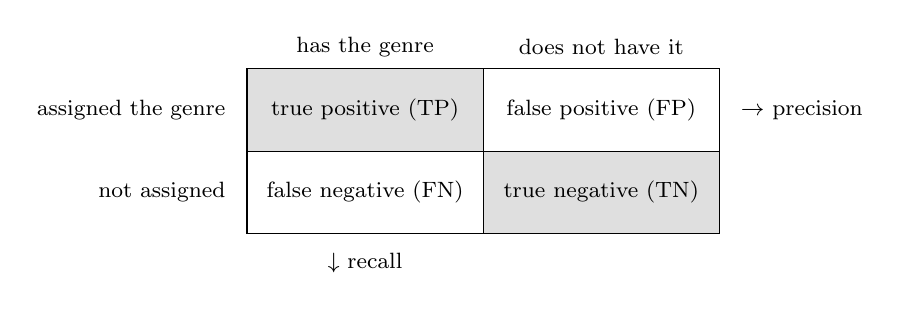
\begin{tikzpicture}[font=\footnotesize,
      cell/.style={draw, minimum width=3.0cm, minimum height=1.05cm, align=center}]
    \node[cell, fill=gray!25] at (0,0) {true positive (TP)};
    \node[cell] at (3.0,0) {false positive (FP)};
    \node[cell] at (0,-1.05) {false negative (FN)};
    \node[cell, fill=gray!25] at (3.0,-1.05) {true negative (TN)};
    \node at (0,0.8) {has the genre};
    \node at (3.0,0.8) {does not have it};
    \node[anchor=east] at (-1.65,0) {assigned the genre};
    \node[anchor=east] at (-1.65,-1.05) {not assigned};
    \node[anchor=west] at (4.65,0) {$\rightarrow$ precision};
    \node at (0,-1.95) {$\downarrow$ recall};
  \end{tikzpicture}
  \caption{The four outcomes of a decision for one genre.}
  \label{fig:confusion}
\end{figure}

In Figure~\ref{fig:confusion}, the columns give the truth and the rows the decision. Precision is read along the first row and recall down the first column:
\begin{equation}
  \text{precision} = \frac{\mathrm{TP}}{\mathrm{TP} + \mathrm{FP}}, \qquad
  \text{recall} = \frac{\mathrm{TP}}{\mathrm{TP} + \mathrm{FN}}, \qquad
  F_1 = \frac{2 \cdot \text{precision} \cdot \text{recall}}{\text{precision} + \text{recall}}.
\end{equation}
Precision is the share of items given the genre that really have it. Recall is the share of items that really have the genre that were given it. $F_1$ is their harmonic mean, so it is high only when both are high. None of the three uses the true negatives. \emph{Macro} averaging computes $F_1$ for each genre and averages these values with equal weight:
\begin{equation}
  \text{macro-}F_1 = \frac{1}{G} \sum_{g=1}^{G} F_{1,g},
\end{equation}
where

\smallskip
\noindent\begin{tabular}{@{}p{0.17\linewidth}p{0.79\linewidth}@{}}
  TP, FP, FN & the numbers of true positives, false positives and false negatives of one genre \\
  $G$ & the number of genres \\
  $F_{1,g}$ & the $F_1$ score of genre $g$ \\
\end{tabular}
\smallskip

\noindent A rare genre therefore counts as much as a common one. This is the standard choice when classes are unbalanced \citep{sokolova2009systematic}. Measures that pool the decisions of all genres, or score whole label vectors, can be misleading there. \emph{Hamming loss} is the share of wrong genre decisions, and \emph{exact match} the share of items whose whole label vector is correct. A trivial classifier that always predicts only the most frequent genre makes few positive predictions and so few false alarms, and it can score better on both than a trained model. Macro-$F_1$ does not have this weakness. A genre that a classifier never predicts receives an $F_1$ of zero, which lowers the average.

\paragraph{Chance level.} Every score is reported against a floor, and the literature uses two different floors. The \emph{most-frequent} baseline predicts, for each genre, whatever is most common in the training data. The \emph{random-guess} baseline ignores the audio altogether. For each film and each genre it draws a random number and assigns the genre with a probability equal to the share of films that carry it. Take the five genres used in most of this thesis (Section~\ref{subsec:genre_labels}). Drama applies to 29 of the 40 films, so the baseline assigns Drama with a probability of 0.725. Comedy applies to 4 films, so the baseline assigns Comedy with a probability of 0.10. The baseline uses no information about a film, so its precision for a genre equals that share. Its recall equals the share as well, because it selects that share of the films that have the genre. Its $F_1$ for the genre is therefore about the share too, and its macro-$F_1$ is about the mean of the shares:
\begin{equation}
  \text{macro-}F_1^{\,\text{random}} \approx \frac{1}{G} \sum_{g=1}^{G} p_g = \frac{0.30 + 0.30 + 0.725 + 0.10 + 0.125}{5} = 0.31,
\end{equation}
where $p_g$ is the share of films that carry genre $g$. For macro-$F_1$ the random-guess floor is the higher of the two, because the most-frequent baseline scores zero on every genre it never predicts. A margin quoted against the lower floor therefore overstates a result.

\paragraph{Without a threshold: ROC-AUC.} $F_1$ needs a yes or no for every genre, so it depends on where the predicted probability is cut. The area under the receiver operating characteristic curve (ROC-AUC) ignores the cut and looks only at the order of the probabilities. It is a ranking test, not a test of decisions. For one genre, it is the probability that a randomly chosen film with the genre receives a higher predicted probability than a randomly chosen film without it:
\begin{equation}
  \text{ROC-AUC} = \frac{1}{n_{+}\, n_{-}} \sum_{i=1}^{n_{+}} \sum_{j=1}^{n_{-}} \left[ \mathbbm{1}(s_i > s_j) + \tfrac{1}{2}\, \mathbbm{1}(s_i = s_j) \right],
\end{equation}
where

\smallskip
\noindent\begin{tabular}{@{}p{0.17\linewidth}p{0.79\linewidth}@{}}
  $n_{+}$, $n_{-}$ & the numbers of films with and without the genre \\
  $s_i$, $s_j$ & the predicted probabilities of a film $i$ with the genre and a film $j$ without it \\
  $\mathbbm{1}(\cdot)$ & 1 if the condition in brackets holds, and 0 otherwise \\
\end{tabular}
\smallskip

\noindent  A value of 1.0 means that this holds for every such pair, so the ranking is perfect. A value of 0.5 means that it holds for half of the pairs, which is what a random ordering achieves on average.

Table~\ref{tab:auc_example} shows a small example with five films, two of which are Horror.

\begin{table}[!htb]
  \centering
  \small
  \caption{A five-film example of ROC-AUC for the genre Horror.}
  \label{tab:auc_example}
  \begin{tabular}{lccc}
    \toprule
    Film & Horror & Predicted probability & Pairs won \\
    \midrule
    A & yes & 0.70 & 3 of 3 \\
    B & no  & 0.60 & -- \\
    C & yes & 0.40 & 2 of 3 \\
    D & no  & 0.30 & -- \\
    E & no  & 0.20 & -- \\
    \midrule
    \multicolumn{3}{l}{Correctly ordered pairs} & 5 of 6 \\
    \bottomrule
  \end{tabular}
\end{table}

In Table~\ref{tab:auc_example}, each Horror film is paired with each of the three other films, which gives six pairs. ``Pairs won'' counts the pairs in which the Horror film has the higher probability. Film A is ranked above all three others. Film C is ranked above D and E but below B. Five of the six pairs are therefore ordered correctly, and the ROC-AUC is $5/6 \approx 0.83$. At a threshold of 0.5, the same model calls only film A Horror and misses film C, so its $F_1$ is modest. Its ranking, however, is good. Moving the threshold changes $F_1$, but it cannot change the ROC-AUC.

A classifier that gives every film the same probability cannot rank at all. In every pair the two films are tied, and a tie counts as half right. Its ROC-AUC is therefore exactly 0.5. This holds for a classifier that assigns every genre to every film, whose $F_1$ can still look good, and equally for one that always predicts ``Drama''. The all-positive classifier has a recall of 1 and a precision equal to the share $p$ of items with the genre, so its $F_1$ is
\begin{equation}
  F_1^{\,\text{all}} = \frac{2 \cdot p \cdot 1}{p + 1} = \frac{2p}{1+p}.
\end{equation} Like $F_1$, the ROC-AUC is computed per genre and then averaged over the genres. It shows whether a model ranks the correct films first, even when its threshold is badly placed. The name comes from the ROC curve, which plots the share of true films found against the share of false alarms for every possible threshold. The area under this curve equals the share of correctly ordered pairs. Every measure that requires a decision can thus be satisfied by some trivial classifier, while ROC-AUC alone says nothing about the decisions a model makes, so the two are best read together.

\subsection{Effect Size: Cohen's $d$}

Several analyses do not evaluate a model but test whether an emotion differs between genres, for example whether fear is higher in Horror clips than in the rest. Cohen's $d$ expresses such a difference in units of the pooled standard deviation:
\begin{equation}
  d = \frac{\bar{x}_{g} - \bar{x}_{\neg g}}{s_p}, \qquad
  s_p = \sqrt{\frac{(n_{g}-1)\,s_{g}^2 + (n_{\neg g}-1)\,s_{\neg g}^2}{n_{g} + n_{\neg g} - 2}},
\end{equation}
where

\smallskip
\noindent\begin{tabular}{@{}p{0.17\linewidth}p{0.79\linewidth}@{}}
  $g$ & the genre under consideration, for example Horror \\
  $\bar{x}_{g}$ & the mean rating of the emotion over the clips of genre $g$ \\
  $\bar{x}_{\neg g}$ & the same mean over all other clips \\
  $s_{g}$, $s_{\neg g}$ & the standard deviation of the rating in each of the two groups \\
  $n_{g}$, $n_{\neg g}$ & the number of clips in each of the two groups \\
  $s_p$ & the pooled standard deviation: the two spreads combined, each weighted by the size of its group \\
  $d$ & the effect size: how far apart the two means are, measured in standard deviations \\
\end{tabular}
\smallskip

\noindent A positive $d$ means the emotion is rated higher in the genre than outside it. Because the difference is divided by the spread of the ratings, $d$ can be compared across emotions whose scales are used differently. By convention, $|d| \approx 0.2$ is a small effect, $0.5$ a medium one and $0.8$ a large one. Fear in Horror, for example, reaches $d = +0.75$. The genre signatures quoted in Section~\ref{par:methods_eight} and reported in Section~\ref{sec:eval_signatures} are given in these units.

\subsection{Statistical Significance Between Models}

Two models are often only a few hundredths of an $F_1$ point apart, and with 40 films such a gap can arise by chance. Two tests are used to assess it, and they answer different questions. In this thesis the bootstrap is the main test for every comparison, and the corrected $t$-test is a stricter check beside it (Section~\ref{subsec:protocol_metrics}).

\paragraph{Paired bootstrap over films.} The first test asks whether a difference would hold if the dataset had held a different sample of films. A new set of test films is drawn from the existing ones with replacement, so some films appear twice and others not at all. Both models are scored on this set, using the predictions they already made, and the difference is recorded. Doing this many times gives a distribution of the difference. Its central 95\,\% is the confidence interval (CI). The two-sided $p$-value is twice the share of draws in which the difference is zero or points the other way. Whole films are drawn, never single clips, because the clips of a film are not independent of each other. An example from Chapter~\ref{ch:evaluation} shows how to read it. On the 40 films, the emotion pipeline scores 0.093 higher than direct VGGish. Over the 2000 draws, the central 95\,\% of the difference runs from $-0.001$ to $+0.191$. In 2.6\,\% of the draws the difference is zero or negative, so $p=0.052$. The lead may well be real, but another sample of films could still eliminate it.

\paragraph{Corrected paired $t$-test.} The second test asks whether the difference would hold with other training data. Repeated cross-validation gives one score per test fold for each model. An ordinary paired $t$-test on these differences would treat them as independent. However, the folds share most of their training films, so it would underestimate the variance and call differences significant too easily. \citet{nadeau2003inference} correct the variance for this overlap (the Nadeau--Bengio test, NB in the tables):
\begin{equation}
  t = \frac{\bar{d}}{\sqrt{\left(\frac{1}{J} + \frac{n_\text{test}}{n_\text{train}}\right)\hat{\sigma}^2}},
\end{equation}
where

\smallskip
\noindent\begin{tabular}{@{}p{0.17\linewidth}p{0.79\linewidth}@{}}
  $J$ & the number of test folds, $50$ (ten repeats of five folds) \\
  $\bar{d}$ & the mean difference in score between the two models over the $J$ folds \\
  $\hat{\sigma}^2$ & the variance of these differences, i.e.\ how much they vary from fold to fold \\
  $n_\text{test}/n_\text{train}$ & the size of a test fold relative to its training set, $1/4$ for five folds \\
  $t$ & the test statistic: the larger $|t|$, the less likely the difference is due to chance \\
\end{tabular}
\smallskip

\noindent The term $1/J$ is the one an ordinary paired $t$-test has, and it shrinks as more folds are added. The term $n_\text{test}/n_\text{train}$ is the correction for the overlapping training sets. The $p$-value is read from a $t$-distribution with $J-1$ degrees of freedom. The added term does not shrink as more repeats are run. This makes the test conservative and puts a lower limit on the $p$-value it can reach on a given dataset (Appendix~\ref{sec:app_comparisons}). The test needs one score per test fold. I therefore use it for the comparisons scored over clips, where every fold has such a score (Section~\ref{subsec:protocol_metrics}).

\paragraph{Many tests at once.} When many comparisons are read together, some reach $p<0.05$ by chance alone. With 18 tests and no real difference, about one such result is expected. The \emph{Holm method} \citep{holm1979simple} guards against this. It sorts the $p$-values from smallest to largest. The smallest is multiplied by the number of tests, the next by one less, and so on, and no adjusted value may be smaller than the one before it. A comparison counts as significant only if its adjusted value stays below 0.05. With 18 tests, a smallest $p$-value of 0.003 thus becomes 0.054.
